
\newcommand{\md}{\cod{md-bbb-{\em version}.img}}
\newcommand{\mdev}{\cod{md-bbb-devel-{\em version}.tar.gz}}
\title[Boot]{Boot \& SD-Karten\\die verschiedenen Möglichkeiten}


\section{Boot}
\begin{frame}{\target} {Die Boot Devices}
  \begin{description}
   \item[SPI0] {\bf S}erial {\bf P}eripheral {\bf I}nterface
   \item[MMC1] die eingebaute SD-Card 
   \item[MMC0] die externe SD-Card \alert{Unser Image}
   \item[UART0] die serielle Schnittstelle
   \item[USB0] USB Schnittstelle
  \end{description}
\end{frame}

\begin{frame}{\target}{zwei Möglichkeiten}
\begin{columns}
\begin{column}{0.5\textwidth}
 \begin{itemize}
  \item die normale:
   \begin{itemize}
    \item \cod{MMC1}, \cod{MMC0}, \cod{UART0}, \cod{USB0}
   \end{itemize}
   \item Boot Switch
   \begin{itemize}
    \item \cod{SPI0}, \cod{MMC0}, \cod{USB0}, \cod{UART0}
   \end{itemize}
 \end{itemize}
\end{column}
\begin{column}{0.5\textwidth}
 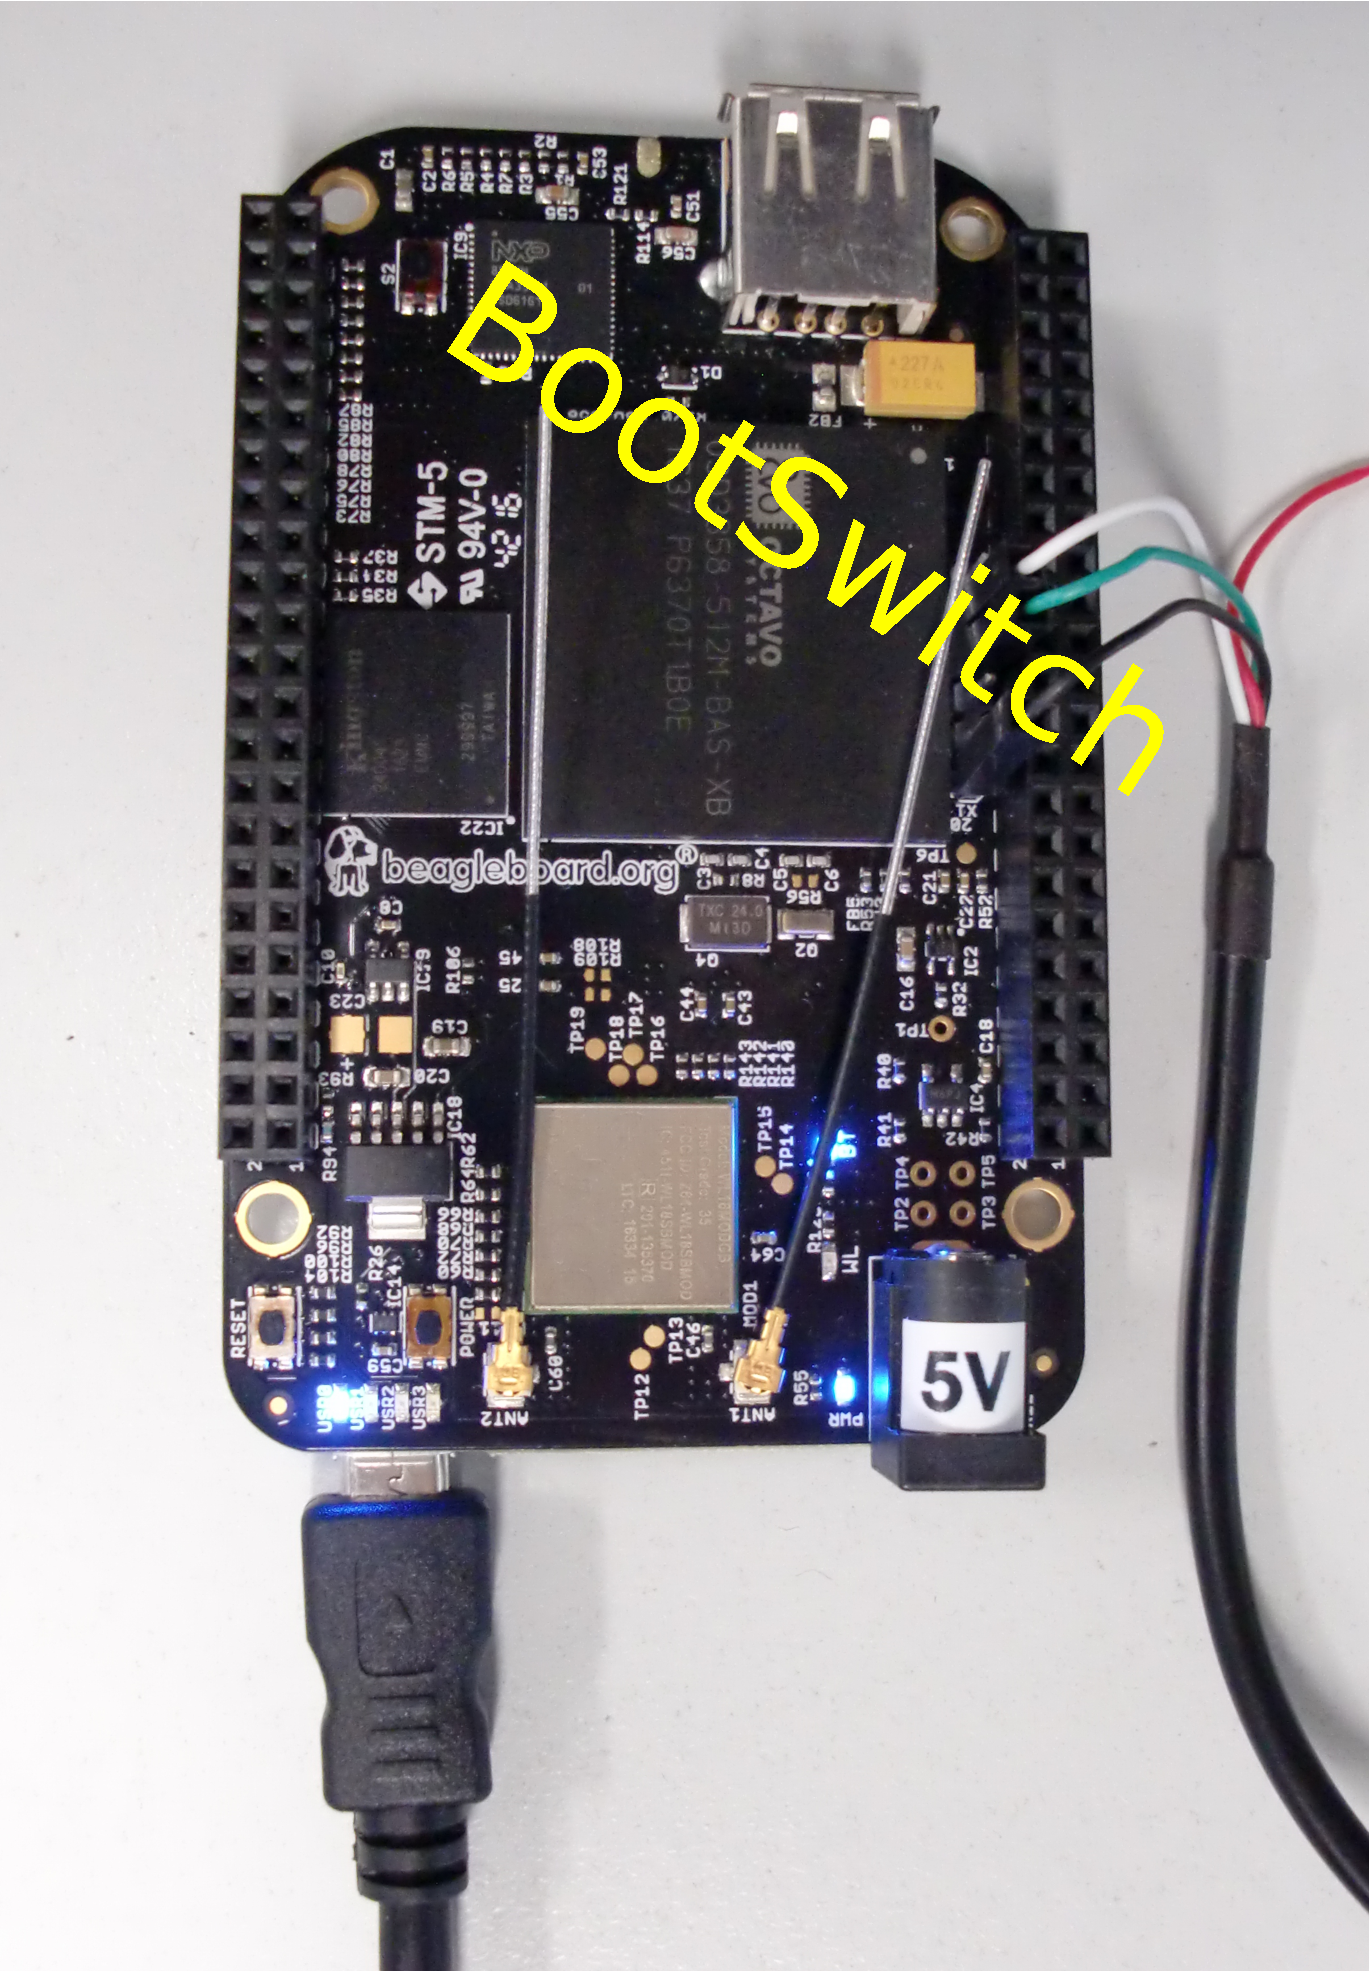
\includegraphics[width=0.75\textwidth]{bbb-boot.pdf}
\end{column}
\end{columns} 
\end{frame}

